\section{Methodology}\label{sec:Methodology}

The methodology used in this research is summarized in the flowchart in \textbf{Figure \ref{fig:CH03_Methodology}}. 

\begin{figure}[h]
    \centering
    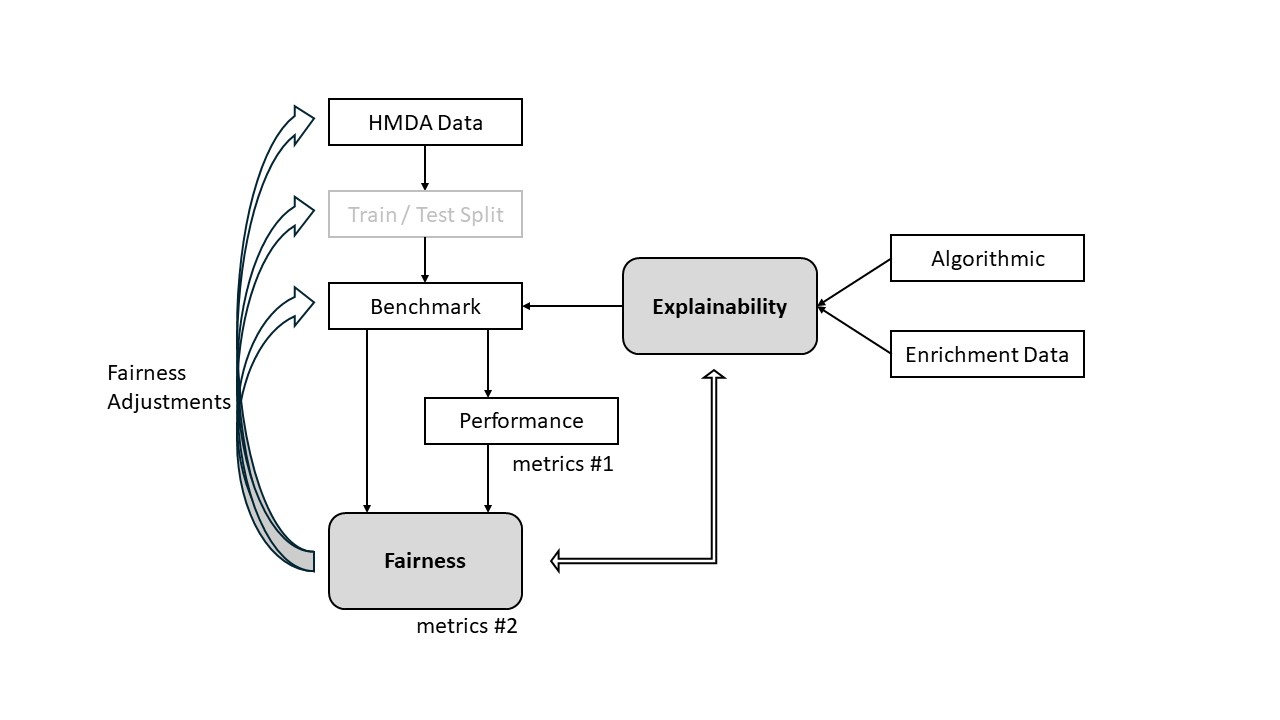
\includegraphics[width=0.85\textwidth]{CH03_Methodology.jpg}
    \caption{Methodology}
    \label{fig:CH03_Methodology}
\end{figure}

Data Preparation and Splitting have already been discussed in \textbf{Chapter \ref{subsec:Data_Preparation}}, details on the remaining steps will be provided in the following.

\subsection{Model Training and Prediction}\label{subsec:Model_Training_and_Prediction}

The model chosen is a comparably simple sequential neural network, implemented with the keras package. Model details are provided in \textbf{Table \ref{tab:CH03_Model_Details}}.

\begin{table}[h]
    \centering
    \begin{tabularx}{\textwidth}{lXr}
    \hline
    \textbf{Layer (type)} & \textbf{Output Shape} & \textbf{Param \#} \\
    \hline
    dense & (None, 32) & 640 \\
    dense\_1 & (None, 64) & 2112 \\
    dropout & (None, 64) & 0 \\
    dense\_2 & (None, 128) & 8320 \\
    dropout\_1 & (None, 128) & 0 \\
    dense\_3 & (None, 64) & 8256 \\
    dropout\_2 & (None, 64) & 0 \\
    dense\_4 & (None, 1) & 65 \\
    \hline
    \textbf{Total params} & & 19,393 \\
    \textbf{Trainable params} & & 19,393 \\
    \textbf{Non-trainable params} & & 0 \\
    \hline
    \end{tabularx}
    \caption{Summary of the Neural Network}
    \label{tab:CH03_Model_Details}
\end{table}



To increase the efficiency of the training process and to prevent overfitting, \textit{callbacks} for early stopping (with a patience of 5 iterations) and best model selection, both based on the validation loss, have been implemented. 
\textit{Adam} is chosen as the optimizer, loss evaluation is based on \textit{categorical crossentropy}, and \textit{accuracy} is selected as the target metric. Training takes place with a batch size of 48 and for a maximum of 30 epochs. 

% Comment on debt_to_income_ratio imputation impacting accuracy but benefitting fairness (after reweighing)

\subsection{Explainability}\label{subsec:Explainability}

% Algorithm choice: Choice of model, reasoning, details of application
% Comment on SHAP and LIME disagreement and add https://arxiv.org/pdf/2202.01602.pdf
% Enrichment data: Explain use of geographical detail 

\subsection{Performance Assessment}\label{subsec:Performance_Assessment}

% Metrics: Choice of metrics, reasoning, details of application
% Cross-validation(?): Choice of method, reasoning, details of application

% Get comparable papers!

\subsection{Fairness Assessment}\label{subsec:Fairness_Assessment}

% Metrics: Choice of metrics, reasoning, details of application

\subsection{Iterations}\label{subsec:Iterations}

% Maybe more detail when decision has actually been made?
% Workflow idea: Training (unadjusted) -> Explainability -> Performance -> Fairness by using aequitas outcome (or checking AIF360) -> new technique by AIF 360 -> aim for similar performance but better fairness